% The "%" character denotes a comment
\documentclass[prb,preprint]{revtex4-1}

\newcommand{\dev}{LSM9DS1} % use "\dev" so you don't have to type LSM9DS1 every time

\begin{document}
\title{Microprocessors - Lab 05 Magnetometer Project (Final Project)}
\author{Adam Stammer}
%\email{adam.stammer@go.winona.edu}

\date{\today}

%if you include an abstract, it goes here
\begin{abstract}
Since my final project parts haven't arrived, I went ahead and used the magnetometer from the \dev to build a different project instead. After getting the magnetometer properly setup and outputting to an LCD screen, I added logic that checked for a magnet above or beneath the sensor, and it's orientation on the plane parallel to the ground. The intent here is that the \dev could be mounted underneath a desk, and a magnet placed above the desk might act as a switch. This could be used with in a direct arduino project, but I took it a step further and wrote a python script that uses the Serial communication to transmit this 'switch' status to a computer. With further development, this could be used to control any number of things on a computer, and the switch can even be disguised/hidden.
\end{abstract}

\maketitle
%title page ends here




\section{Magnetometer Readout}
Since I was able to use my previous lab code as a starting point, it was quite easy to switch the data being printed and used from the accelerometer to the magnetometer. This quickly got me magnetometer readings straight to the LCD. If you want to know more on the setup that that entails, see my previous Lab 05 report. The datasheet axis diagram can be see below.

\begin{figure}[H]
	\centering
	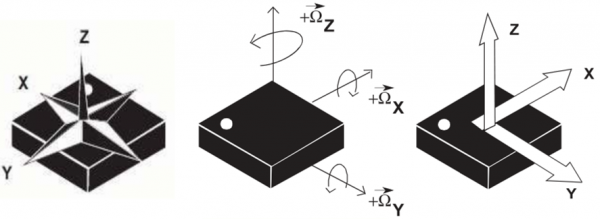
\includegraphics[width=5.75in]{axes.png}
	\caption{\dev  Axis Orientation}
	\label{fig1}
\end{figure}

\section{Magnet Detection}
From here, I mounted the \dev board underneath my monitor stand. I could've used my desk but the monitor stand made it easier to mount without bending wires too much. If this project was to be truly installed on my desk, I would've also mounted the arduino, which would've removed the wiring issue. Either way the concepts are the same. For reference, my monitor stand is about 3/4" thick pine wood. 

With the board mounted and measurements being printed out I simply compared the measurements with and without a magnet sitting directly above the board. As the diagram in the datasheet suggests, the Z axis showed a massive jump from <1 to >4 when I placed the magnet. This makes sense as the magnet creates a magnetic field vertical to the magnetometer regardless of the magnet's orientation. For reference I used the Handi-Pack 7/8" x 3/16" Bar Magnet (Part \# 85783) because I had one lying around, and it's strong enough and small enough to fit the requirements of this project. Depending on whether or not the board is mounted upside down, will determine the polarity of this change in Z. Just to be safe I used the absolute value function in the arduino in my logic checks. I used the same LED setup from my previous labs to indicate a magnet being present, and also printed a message to the LCD ("MAG" or "NO MAG").

Thankfully, at less than an inch away, the magnetic field of my bar magnet was much stronger than that of the Earth. If the magnet was too weak, this detection might not work at this range. As it was, I was pretty much able to ignore the magnetic field of the Earth entirely.


\section{Magnet Orientation}
Next, I wanted to determine which direction the magnet was laying. I decided that just two orientations good enough, parallel to either the X or the Y axis. Without too much work one could add additional orientations between these two, but it didn't seem very realistic, since I was aiming for a switch, not a dial. Again, looking at the readouts, it was clear that whichever axis was parallel to the bar magnet had much stronger readings than the other. The only catch here was that which direction the north and south poles were facing determined the polarity of these X and Y axis measurements. I didn't want the magnet poles to be forced one direction or the other as that can get confusing, especially since they aren't marked, so again I just used the absolute value function to simply look at the magnitude of each measurement. Then a simple inequality was used to decide which axis had a stronger reading, which then activated the respective orientation flag. This gave me three possible states: Orientation 1, Orientation 2, or No Magnet. Again, I changed the LCD message to reflect this. The red LED would turn on unless the magnet was not present still, though this was for testing purposes and wouldn't make sense in a real installation of this project. 

\section{Desktop Interfacing}
The switch could be used as a switch in any existing microcontroller project, but I've always wanted to connect this kind of thing to my desktop. Hide the magnet in the bottom of some desk bauble like an action figure or a pencil sharpener, and have my desktop PC react to that devices presence/orientation. I had the input information, I just needed to get it to the PC. This proved more of a challenge than I imagined, because Serial communication varies greatly from one operating system to the next. I first tried writing a program in Java to accomplish this, but quickly gave up as everyone online suggested to not use Serial in Java, and any example code I could find using the COM ports was many pages long. C++ was my next thought, but I didn't expect it to be easier than Java. A quick google search said I was right. Since quick development was obviously the goal I finally thought of Python. In a true installation of this project I would likely try to figure out the extensive COM procedures in C++, but for the sake of testing I'm glad I went with Python.

I managed to find the pySerial module (\url{https://pythonhosted.org/pyserial/pyserial.html}), which allowed me to open and read from a COM port in very little code. Since serial is implemented so differently from one operating system to the next, one would have to either write code for each operating system or code in some operating system check (much harder than it should be btw), but I don't think this kind of project would ever be very mass production feasible. The installation, various types of magnets, different desk thicknesses and materials, etc. make this kind of thing much too case by case. Perhaps with a very clear installation guide, and a lot of very user friendly code, it could be done, but I think it would be difficult for most non-technical people to setup themselves. As such I figure the code would be written by the one installing the project, so I just wrote my code for Windows. This is meant to be a proof of concept at this point anyway.

With the Serial port open and data being read, I added some if statements, though a switch/case would've served the same purpose. The arduino was sending a message based on the orientation: ORIENT1, ORIENT2, NO MAG. The only other possible input was an empty string if the serial read timed out, though this was simply ignored. As a proof of concept, I just output the status to the screen, though the code within these if statements could be changed to whatever a person wanted. Anything that you can do with python could be controlled with this kind of program. If you've ever heard of the program suite called If This Then That (ITTT), you can see that a program can have a lot of power over ones computer. I believe that ITTT even has input interfacing with most of the major programming languages, including python, so if one wanted to simplify this process, and avoid code, you could use this python script to send a message to the ITTT PC client, and use the ITTT gui to program its response from there. I'd have to look more into ITTT to be sure, but I've heard some very good things about it. 

I didn't want to embed my magnet into something just yet, so instead I tossed it inside an empty pill bottle I had handy. By sheer luck, it was an iron supplement bottle. A video of the current state of this project can be found at \url{https://mediaspace.minnstate.edu/media/3+State+Magnet+Switch+Demo/1_w8qs7oln}. I'll have to get a magnetometer of my own, but I do plan to continue this project. Perhaps if I open the idea to the internet, others will have more practical applications than I currently do. 

%\begin{thebibliography}{99}
% The numeral (here 99) in curly braces is nominally the number of entries in
% the bibliography. It's supposed to affect the amount of space around the
% numerical labels, so only the number of digits should matter--and even that
% seems to make no discernible difference.
%Not Requested
%\end{thebibliography}

\end{document}
